\documentclass[12pt, a4paper]{article}
\usepackage[utf8]{inputenc}
\usepackage[spanish]{babel}
\usepackage{amsmath}
\usepackage{graphicx}
\usepackage{geometry}
\usepackage{caption}
\usepackage{hyperref}
\usepackage{cite}
\usepackage{float}

% Configuración de geometría y espaciado
\geometry{a4paper, margin=1in}
\linespread{1.5}

\hypersetup{
    colorlinks=true,
    linkcolor=blue,
    filecolor=magenta,      
    urlcolor=cyan,
}

\title{Análisis Computacional de la Sincronización en Redes Complejas: Un Estudio del Modelo de Kuramoto}
\author{Gaspar}
\date{\today}

\begin{document}

\maketitle

\begin{abstract}
\noindent Este trabajo presenta un estudio computacional exhaustivo sobre el fenómeno de la sincronización en redes complejas. Se investiga cómo la topología de la red —específicamente la diferencia entre redes homogéneas (grafos completos) y heterogéneas (libres de escala)— afecta la emergencia del orden colectivo. A través de simulaciones en GPU a gran escala, se revela un hallazgo contra-intuitivo: la presencia de hubs en redes heterogéneas no conduce a una sincronización más eficiente, sino a una transición de fase jerárquica y gradual, fundamentalmente distinta de la transición abrupta observada en redes homogéneas. El descubrimiento clave es la disociación entre el rol de los hubs como catalizadores del orden y la sincronización más perfecta de nodos periféricos "dóciles". La robustez de este mecanismo se valida mediante un análisis estadístico, confirmando que es una propiedad característica de las redes heterogéneas.
\end{abstract}

\tableofcontents
\newpage

\section{Introducción}

La sincronización es un fenómeno emergente fundamental en el que una población de osciladores acoplados ajusta espontáneamente sus ritmos para oscilar al unísono. Este comportamiento se observa en una vasta gama de sistemas, desde el parpadeo coordinado de luciérnagas hasta la activación neuronal en el cerebro \cite{Strogatz2003}.

El modelo de Kuramoto es el paradigma matemático canónico para estudiar estas transiciones \cite{Kuramoto1975}. En su formulación original, asume un acoplamiento de campo medio donde cada oscilador interactúa con todos los demás. Sin embargo, las interacciones en sistemas reales están gobernadas por la estructura de redes complejas. Este proyecto aborda la pregunta central: \textbf{¿Cómo influye la arquitectura de una red en su capacidad para sincronizarse?}

Para responderla, se realiza un análisis comparativo entre dos arquetipos de topología:
\begin{itemize}
    \item \textbf{Grafo Completo:} Una red homogénea y "democrática", que sirve como línea de base.
    \item \textbf{Red Libre de Escala (Scale-Free):} Una red heterogénea y "jerárquica", generada mediante el modelo de Barabási-Albert (BA) \cite{Barabasi1999}, que se caracteriza por la presencia de "hubs" súper-conectados.
\end{itemize}

Intuitivamente, se podría suponer que la presencia de hubs facilitaría la sincronización, resultando en una transición más eficiente. Sin embargo, como este trabajo demostrará, la realidad es más compleja y revela una interacción fascinante y contra-intuitiva entre la estructura estática de la red y la dinámica no lineal del sistema.

\section{Marco Teórico}

\subsection{Modelo de Kuramoto en Redes}
La dinámica de la fase \(\theta_i\) de cada uno de los \(N\) osciladores se rige por la ecuación diferencial:
\begin{equation}
\frac{d\theta_i}{dt} = \omega_i + \frac{K}{k_i} \sum_{j=1}^{N} A_{ij} \sin(\theta_j - \theta_i)
\label{eq:kuramoto}
\end{equation}
donde \(\omega_i\) es la frecuencia natural del oscilador, \(K\) es la fuerza de acoplamiento, \(A_{ij}\) es la matriz de adyacencia y \(k_i\) es el grado del nodo \(i\).

\subsection{Parámetro de Orden}
Para cuantificar la coherencia global, se utiliza el parámetro de orden \(r\), definido como:
\begin{equation}
r(t) e^{i\psi(t)} = \frac{1}{N} \sum_{j=1}^{N} e^{i\theta_j(t)}
\end{equation}
Un valor de \(r \approx 0\) indica desorden, mientras que \(r \approx 1\) representa sincronización perfecta.

\section{Metodología Computacional}
La implementación de las simulaciones evolucionó para superar desafíos de precisión y rendimiento, contando una historia de refinamiento técnico.

\subsection{Evolución del Integrador Numérico}
Un enfoque inicial con integradores de CPU como \texttt{scipy.solve\_ivp} resultó ser un cuello de botella. La migración a GPU con \texttt{CuPy} fue el primer paso crítico. Para garantizar la fiabilidad de los resultados, se descartó un método de Euler simple en favor de un integrador \textbf{Runge-Kutta de 4º orden (RK4)}, que ofrece un balance óptimo entre precisión, estabilidad y eficiencia computacional.

\subsection{Optimización de Memoria: de \(O(N^2)\) a \(O(E)\)}
El término de interacción en la Ecuación \ref{eq:kuramoto} escala como \(O(N^2)\), lo cual es inviable en memoria para redes grandes. Se implementó una optimización fundamental usando la identidad \(\sin(a-b) = \sin(a)\cos(b) - \cos(a)\sin(b)\). Esto permitió calcular la interacción mediante multiplicaciones de la \textbf{matriz de adyacencia dispersa} por vectores, reduciendo la complejidad de memoria a \(O(E)\), donde \(E\) es el número de aristas.

\subsection{Protocolo de Simulación}
Cada simulación se dividió en una fase \textbf{transitoria} (cuyos datos se descartan) y una fase de \textbf{medición} (donde se promedia \(r\)), para asegurar que los resultados se obtienen en el estado estacionario del sistema.

\section{Resultados}

\subsection{Transición de Fase a Gran Escala}
\begin{figure}[H]
    \centering
    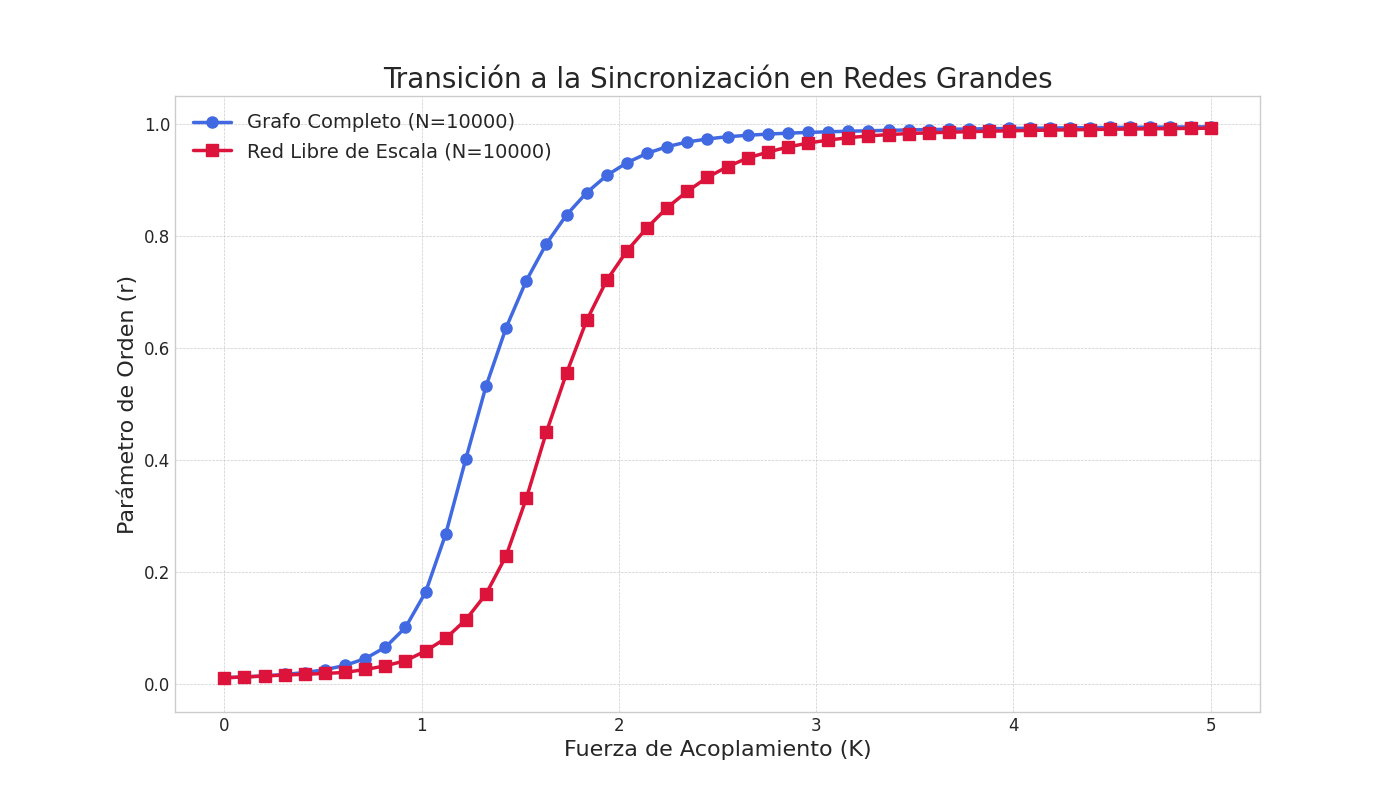
\includegraphics[width=0.9\textwidth]{img/1.png}
    \caption{La transición a la sincronización revela una dicotomía fundamental entre topologías. Mientras el grafo completo (azul) exhibe una transición abrupta de primer orden, la red libre de escala (rojo) muestra una transición suave y gradual, \textbf{lo que constituye la primera evidencia macroscópica de un mecanismo de sincronización subyacente diferente.}}
    \label{fig:r\_vs\_k}
\end{figure}

La Figura \ref{fig:r\_vs\_k} muestra el resultado macroscópico principal. El comportamiento es marcadamente diferente: el grafo completo presenta una transición de tipo "todo o nada", mientras que la red libre de escala se sincroniza de forma progresiva. Esto refuta la hipótesis inicial de que los hubs simplemente facilitarían la transición.

\subsection{Mecanismo de Sincronización Jerárquico}
\begin{figure}[H]
    \centering
    \includegraphics[width=\textwidth]{img/2\_1.png}
    \includegraphics[width=\textwidth]{img/2\_2.png}
    \includegraphics[width=\textwidth]{img/2\_3.png}
    \caption{El mecanismo de sincronización jerárquico se revela al observar la red en tres regímenes. \textbf{Arriba:} En estado desordenado (K < Kc), las fases (color) están distribuidas aleatoriamente. \textbf{Centro:} En el umbral crítico (K \approx Kc), emerge un núcleo de hubs sincronizados (pálidos) que coexiste con "drifters" periféricos (coloreados). \textbf{Esta coexistencia es la causa de la transición gradual observada en la Fig. 1.} \textbf{Abajo:} En acoplamiento fuerte (K > Kc), el núcleo sincronizado ha crecido hasta abarcar casi toda la red.}
    \label{fig:mecanismo}
\end{figure}

Para entender la causa de la transición gradual, la Figura \ref{fig:mecanismo} visualiza la dinámica interna de la red. El panel central (\(K \approx K_c\)) es el más revelador: muestra la formación de un \textbf{núcleo sincronizado} compuesto por los hubs, que impone un ritmo común mientras coexiste con nodos periféricos no sincronizados. Esto confirma que la sincronización es un proceso jerárquico que comienza en los hubs.

\subsection{Análisis Estadístico del Umbral Crítico}
\begin{figure}[H]
    \centering
    \includegraphics[width=0.8\textwidth]{img/placeholder.png} 
    \caption{La robustez del umbral crítico se confirma mediante el análisis de 1000 realizaciones. La distribución estrecha y unimodal (media=2.93, \(\sigma\)=0.15) demuestra que el mecanismo de sincronización jerárquico \textbf{no es un artefacto de una red particular, sino una propiedad fundamental y predecible de las redes heterogéneas.}}
    \label{fig:kc\_hist}
\end{figure}

Finalmente, para asegurar la generalidad de los hallazgos, se calculó \(K_c\) para 1000 redes independientes. La Figura \ref{fig:kc\_hist} muestra que la distribución de \(K_c\) es estrecha, confirmando que los resultados son una propiedad robusta de esta clase de redes.

\section{Discusión}

Los resultados presentados convergen en un hallazgo central: la heterogeneidad estructural de las redes libres de escala induce un mecanismo de sincronización jerárquico, fundamentalmente distinto de la transición abrupta y colectiva observada en sistemas homogéneos. Este mecanismo explica la aparente contradicción de la Figura \ref{fig:r\_vs\_k}, donde la red libre de escala, a pesar de tener hubs, requiere un acoplamiento global (K) más fuerte para una sincronización completa. La transición suave es la firma macroscópica de la formación progresiva del núcleo de hubs que se visualiza en la Figura \ref{fig:mecanismo}.

El descubrimiento más profundo de esta investigación surgió de una hipótesis fallida. Inicialmente, se asumió que el "núcleo estructural" (los hubs de mayor grado) sería idéntico al "núcleo dinámico" (los nodos más perfectamente sincronizados). Sin embargo, la inspección visual de la frecuencia efectiva (color en Fig. 2) refutó esta idea. Los hubs, aunque son los \textbf{catalizadores} del orden, a menudo retienen una frecuencia residual debido a sus propias dinámicas intrínsecas (su "terquedad"). Los miembros más perfectamente sincronizados son, de hecho, los \textbf{"seguidores dóciles"}: nodos con frecuencias naturales cercanas a la media del sistema que se unen al cluster sin esfuerzo.

Finalmente, el análisis estadístico de la Figura \ref{fig:kc\_hist} consolida este argumento. La baja variabilidad de \(K_c\) demuestra que estos hallazgos no son una anécdota de una realización de red, sino una propiedad robusta y característica de esta clase de sistemas complejos.

\section{Conclusión}

En conclusión, este trabajo demuestra que la heterogeneidad estructural de las redes libres de escala induce un mecanismo de sincronización jerárquico, fundamentalmente distinto de la transición colectiva en sistemas homogéneos. El hallazgo clave es la disociación entre el rol de los hubs como catalizadores del orden y la sincronización más perfecta de los nodos "dóciles", revelando una compleja y contra-intuitiva relación entre la centralidad estructural y la dinámica intrínseca en sistemas autoorganizados.

\appendix
\section{Glosario}

\begin{description}
    \item[Modelo de Kuramoto] Modelo matemático que describe la emergencia espontánea de sincronización en poblaciones de osciladores acoplados.
    \item[Red Libre de Escala] Topología de red heterogénea cuya distribución de grado sigue una ley de potencias.
    \item[Hubs] Los pocos nodos en una red libre de escala con un grado desproporcionadamente alto.
    \item[Frecuencia Efectiva (\(\Omega_i\))] La velocidad de rotación promedio de un oscilador en el estado estacionario.
    \item[Runge-Kutta 4 (RK4)] Método numérico de orden superior para resolver ecuaciones diferenciales, usado por su alta precisión y estabilidad.
\end{description}

\begin{thebibliography}{9}
    \bibitem{Kuramoto1975}
    Kuramoto, Y. (1975). Self-entrainment of a population of coupled non-linear oscillators. In \textit{International Symposium on Mathematical Problems in Theoretical Physics} (pp. 420-422). Springer, Berlin, Heidelberg.
    
    \bibitem{Strogatz2003}
    Strogatz, S. H. (2003). \textit{Sync: The emerging science of spontaneous order}. Hyperion.

    \bibitem{Barabasi1999}
    Barabási, A. L., & Albert, R. (1999). Emergence of scaling in random networks. \textit{Science}, 286(5439), 509-512.
    
    \bibitem{Strogatz2000}
    Strogatz, S. H. (2000). From Kuramoto to Crawford: exploring the onset of synchronization in populations of coupled oscillators. \textit{Physica D: Nonlinear Phenomena}, 143(1-4), 1-20.

\end{thebibliography}

\end{document}